%==========================================================================================

\documentclass[10pt]{article}

%==========================================================================================

\usepackage[utf8]{inputenc}
\usepackage[brazil]{babel}
\usepackage[T1]{fontenc}
\usepackage{amsmath}
\usepackage{amsfonts}
\usepackage{mathrsfs}
\usepackage{amssymb}
\usepackage{graphicx}
\usepackage{geometry, calc, color, setspace}
\usepackage{indentfirst}
\usepackage{wrapfig}
\usepackage{boxedminipage}
\usepackage{enumerate}
\usepackage{float}
\usepackage[hang]{caption}
\usepackage{paralist}
\usepackage{comment}
\usepackage{icomma}
\usepackage{rotating}
\usepackage{multirow}

\usepackage{array}
\newcolumntype{C}[1]{>{\centering\let\newline\\\arraybackslash\hspace{0pt}}m{#1}}

\usepackage[abnt-substyle=UFLA,abnt-emphasize=bf,abnt-etal-list=3,abnt-and-type=e]{abntcite}

\newcommand{\HRule}{\noindent\rule{\linewidth}{0.2mm}}

\usepackage{mathpazo}                         % tem suporte matemático
\usepackage[scaled=0.85]{beramono}            % usa esta nos verbatins [scaled=0.9]

\def\distnumber{2.3em}

%==========================================================================================

\author{Walmes Marques Zeviani\footnote{Doutorando em Estatística e
Experimentação Agropecuária, DEX/UFLA. Professor do Departamento de Estatística
- UFPR. Contato: walmes@ufpr.br.}}

%==========================================================================================


\title{Uma parametrização do modelo van Genuchten para inferência sobre os parâmetros $S$ e $I$}
\date{}

\begin{document}

\maketitle

\begin{abstract}
A água é indispensável para produção das culturas pois está envolvida
no transporte de nutrientes, reações químicas, processos físicos e
manutenção da vida do solo. O conhecimento sobre a curva de rentenção
de água (CRA) do solo é fundamental para estabelecer estratégias de
manejo. A qualidade física do solo é depende da CRA e os parâmetros
$I$, tensão do ponto de inflexão da CRA, e $S$, taxa de variação no
ponto de inflexão, considerados como indicadores da qualidade física,
são parâmetros relacionados a medidas descritivas da distribuição do
tamanho de poros do solo. Com este trabalho, objetiva-se verificar o
efeito da posição de amostragem e profundidade do solo sobre os
parâmetros $I$ e $S$ da CRA. Para isso 1) considerou-se ANOVA simples
e 2) ANOVA ponderada pela variância das estimativas desses parâmetros
em cada unidade experimental em comparação com 3) o uso de modelos não
lineares de efeito misto em uma parametrização desenvolvida para $I$ e
$S$. Nenhum dos métodos alternativos de análise foi superior ao modelo
não linear de efeitos mistos na parametrização desenvolvida, que
apresentou intervalos mais estreitos para estimativas dos parâmetros e
apontou efeito de posição e profundidade de coleta nos parâmetros $I$
e $S$.\\
\newline
\noindent {Palavras-chave}: Reparametrização. Função de parâmetros. Método delta. Curva de retenção de água.

\end{abstract}

\section{INTRODUÇÃO}

Água é indiscutivelmente o fator isolado mais importante, com possível
exceção para luz solar e o ar que não têm disponibilidade limitada,
para o desenvolvimento das plantas \cite{Chesworth2007}.  A água
presente no solo desempenha inumeráveis funções de ordem química,
física e biológica como, por exemplo, dissolver e transportar
nutrientes para as plantas além de também ser considerada um nutriente
\cite{Brady2009}.  O excesso de água no solo pode diminuir ou impedir
o desenvolvimento das plantas devido a uma reduzida aeração, enquanto
deficiências podem causar estresse hídrico e, se severa o suficiente,
o murchamento e morte da planta. Para uma produção eficiente, um
fornecimento constante de água é necessário durante o ciclo da planta
para atender as necessidades hídricas e promover a dissolução,
transporte e absorção de nutrientes. O conteúdo de água também
influencia a qualidade de operações de manejo do solo e colheita.

\newpage
\section{RETENÇÃO DE ÁGUA E TAMANHO DE POROS}\label{sc-craporos}

Dada a relação que existe entre tamanho de poros e tensão matricial
é possível chegar à distribuição de frequência
de tamanho de poros quando o modelo \citeonline{VanGenuchten1980} é
usado para representar a CRA \cite{Reynolds2002a}. Essa relação não
pode ser considerada isoladamente pois fatores que alteram as
propriedades da água de um solo para o outro a modificam, como a
concentração de íons e a temperatura. Por outro lado, fixadas as
demais variáveis, essa relação permite explorar a conexão existente
entre a retenção de água e distribuição de tamanho de poros. Além do
mais, a partir dessa relação, é possível verificar que o parâmetro $S$
proposto por \citeonline{Dexter2004} é o parâmetro de escala que
representa o grau de dispersão de valores ao redor do tamanho modal de
poros.

\newpage
\section{MATERIAL E MÉTODOS}\label{sc-methods}

Os dados considerados são medidas de conteúdo de água do solo (m$^3$
m$^{-3}$) em função do potencial matricial (kPa) coletados em campo
sob cultura do cafeeiro no qual se utilizam métodos conservacionistas
e de manejo intensivo do solo \cite{Serafim2011}. Amostras de solo
indeformadas foram coletadas de um solo classificado como Latossolo
Vermelho distroférrico (LVd) em uma lavoura com 3,5 anos de
implantação.

\begin{figure}[!ht]
 \begin{center}
 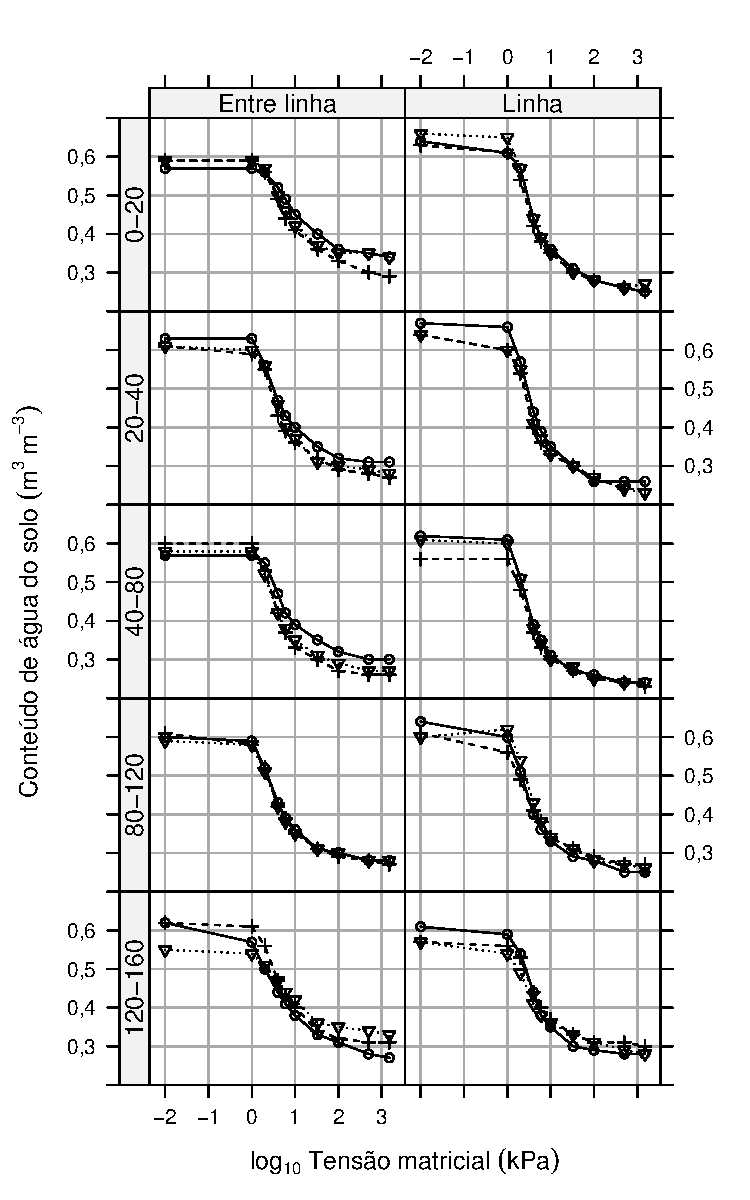
\includegraphics[width=0.7\textwidth]{../figuras/cra_perfil.pdf}
\end{center}
 \caption{Conteúdo de água do solo (m$^3$ m$^{-3}$) em função do
   log$_{10}$ da tensão matricial (kPa) organizado pelas combinações
   entre posição (nas colunas) e profundidade de coleta (nas linhas).
   As três unidades experimentais em cada combinação foram
   identificadas pelos tipos de pontos e linhas}
 \label{fg-craperfil}
\end{figure}

\newpage
\section{RESULTADOS E DISCUSSÃO}\label{sc-results}

Estimativas dos parâmetros foram obtidas para as 30 unidades
experimentais sob as duas parametrizações do modelo van Genuchten.  Os
valores de R$^2$ apontaram boa medida de ajuste pois ficaram entre
98,96\% e 99,88\%.  Pelas estimativas intervalares, considerando os
seis parâmetros definidos pelas duas parametrizações, $U_s$, $U_r$,
$a$, $n$, $S$ e $I$, observamos variação entre unidades experimentais
dentro de uma mesma cela experimental (combinação de posição e
profundidade), entre níveis de profundidade e entre posições de
amostragem (Figura \ref{fg-ICpar}).  Verifica-se que os parâmetros
$U_r$ e $n$, por serem comuns as duas parametrizações, tiveram mesmas
estimativas intervalares independentemente da parametrização.

\begin{figure}[H]
 \begin{center}
 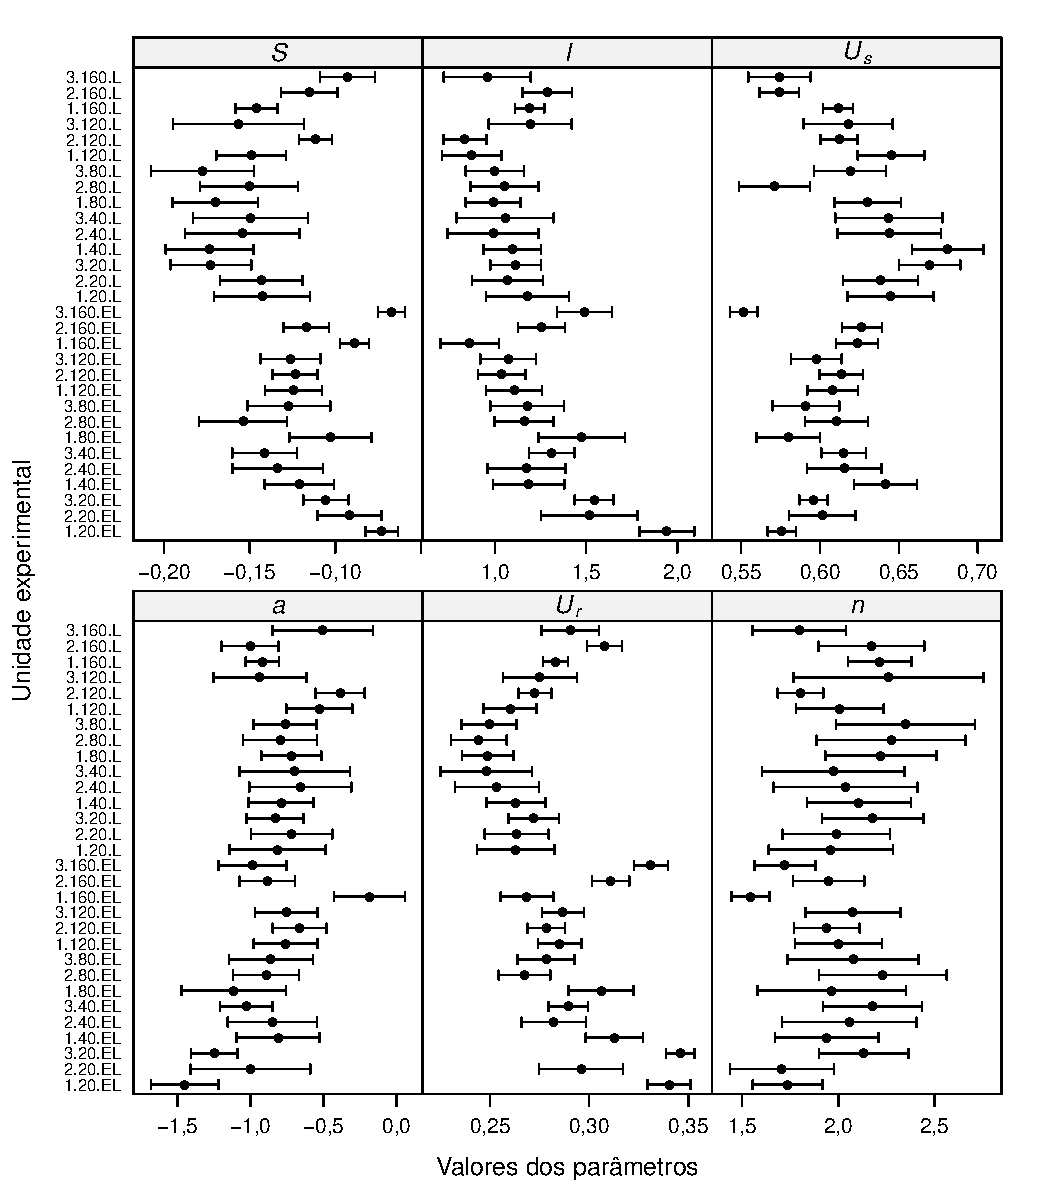
\includegraphics[width=0.8\textwidth]{../figuras/param_ic.pdf}
\end{center}
 \caption{Estimativas intervalares (95\%) pelo método de Wald para os
   parâmetros da CRA considerando as duas parametrizações do modelo
   van Genuchten.  Os rótulos no eixo das coordenadas representam o
   índice da repetição, o nível de profundidade e o nível de posição,
   separados por ponto}
 \label{fg-ICpar}
\end{figure}

\newpage
\section{CONCLUSÕES}\label{sc-conclusion}

Conclui-se que o modelo não linear de efeitos mistos é um método de
análise mais adequado para representar os dados uma vez que toda
informação está contida em um único modelo que permite acomodar os
efeitos de termos fixos e aleatórios, comparar modelos e fazer
predições para a CRA.

\newpage
\addcontentsline{toc}{section}{\hspace*{\distnumber}REFERÊNCIAS}
\begin{center}
\section*{REFERÊNCIAS} 
\end{center}


% Use isso descomentado durante edição.
% Quando concluir a Tese, comente iss e use
% o código do bloco abaixo.
\begin{singlespace}
\renewcommand\refname{}
\begin{flushleft}
\bibliography{../tese/bibtese2}
\end{flushleft}
\end{singlespace}

%% Em cap2nlme-corrigido.bbl foi feita correção manual de
%% algumas referências como por exemplo as citações
%% de Dissertação e Tese.
%% Então deixa-se de usar o arquivo cap2nlme.bbl gerado
%% automaticamente pelo abntcite, mas isso é só ao final.
% \begin{singlespace}
% \begin{flushleft}
% \renewcommand\refname{}
% \vspace*{-1.5cm}
% \input{cap2nlme-corrigido.bbl}
% \end{flushleft}
% \end{singlespace}

\section{Anexos}

\begin{singlespace}
\noindent{{ANEXO A:$\,\,$} Código R reproduzível correspondente ao
ajuste do modelo van Genuchten reparametrizado para inferência sobre os parâmetros $I$ e $S$.
Disponível online
em: \texttt{http://www.leg.ufpr.br/\~{}walmes /TESE/anexoCRA.R}}
\end{singlespace}
\noindent \rule[4mm]{\textwidth}{0.1ex}
\begin{small}
\linespread{0.7}
\vspace{-1cm}
\input{../scripts/anexoCRA.R}
\noindent \rule[4mm]{\textwidth}{0.1ex}
\end{small}

\def\capanexo{Conteúdo de água do solo (m$^3$ m$^{-3}$) em função da tensão matricial (kPa), da profundidade (cm)
 e da unidade experimental (UE) para amostras coletadas na}

\begin{sidewaystable}
 \caption{\capanexo{} entre linha.}\label{tab:anexoEL}
\begin{center}
 \input{../tabelas/anexotabEL.txt}
\end{center}
\end{sidewaystable}

\begin{sidewaystable}
 \caption{\capanexo{} linha.}\label{tab:anexoL}
\begin{center}
 \input{../tabelas/anexotabL.txt}
\end{center}
\end{sidewaystable}

\end{document}

%==========================================================================================
